\definecolor{green}{RGB}{0,128,0}
  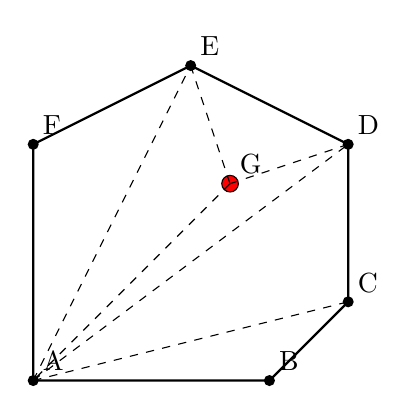
\begin{tikzpicture}
    % Define the points
    \coordinate (A) at (0,0);
    \coordinate (B) at (3,0);
    \coordinate (C) at (4, 1);
    \coordinate (D) at (4,3);
    \coordinate (E) at (2,4);
    \coordinate (F) at (0,3);
    \coordinate (G) at (2.5,2.5);
    
    % Draw the points
    \foreach \point in {A,B,C,D,E,F,G}
      \fill (\point) circle (2pt);

    \onslide<2->{\draw[thick] (A) -- (B) -- (C) -- (D) -- (E) -- (F) -- cycle;}

    % Draw a dashed line between the pivot and the points
    \onslide<3->{
        \draw[dashed] (A) -- (B);
        \draw[dashed] (A) -- (C);
        \draw[dashed] (A) -- (D);
        \draw[dashed] (A) -- (E);
        \draw[dashed] (A) -- (F);
    }

    
    \onslide<4-> {\draw[fill=red] (G) circle (3pt);}
    \onslide<5->{
        \draw[dashed] (G) -- (A);
        \draw[dashed] (G) -- (D);
        \draw[dashed] (G) -- (E);
    }
    
    % Label the points
    \node[above right] at (A) {A};
    \node[above right] at (B) {B};
    \node[above right] at (C) {C};
    \node[above right] at (D) {D};
    \node[above right] at (E) {E};
    \node[above right] at (F) {F};
    \node[above right] at (G) {G};

    \end{tikzpicture}
